\ifx\boi\undefined\ifx\problemname\undefined
\providecommand\sampleinputname{}
\providecommand\sampleoutputname{}
\documentclass[nil]{templates/boi}
\ifdefined\babelprovide
  \babelprovide[import=lv,main]{latvian}
\fi
\problemlanguage{.lv}
\fi
\newcommand{\boi}{Baltijas informātikas olimpiāde}
\newcommand{\practicesession}{Izmēģinājuma kārta}
\newcommand{\contestdates}{27.~aprīlis~-- 1.~maijs, 2018}
\newcommand{\dayone}{1.~diena}
\newcommand{\daytwo}{2.~diena}
\newcommand{\licensingtext}{Šis uzdevums ir licencēts zem CC BY-SA~4.0.}
\newcommand{\problem}{Uzdevums}
\newcommand{\inputsection}{Ievaddati}
\newcommand{\outputsection}{Izvaddati}
\newcommand{\interactivity}{Komunikācija}
\newcommand{\grading}{Testēšana}
\newcommand{\scoring}{Vērtēšana}
\newcommand{\constraints}{Ierobežojumi}
\renewcommand{\sampleinputname}{Ievaddatu paraugs}
\renewcommand{\sampleoutputname}{Izvaddatu paraugs}
\newcommand{\sampleexplanation}[1]{#1.~parauga paskaidrojums}
\newcommand{\sampleexplanations}{Paraugu paskaidrojumi}
\newcommand{\timelimit}{Laika ierobežojums}
\newcommand{\memorylimit}{Atmiņas ierobežojums}
\newcommand{\seconds}{s}
\newcommand{\megabytes}{MB}
\newcommand{\group}{Grupa}
\newcommand{\points}{Punkti}
\newcommand{\limitsname}{Ierobežojumi}
\newcommand{\additionalconstraints}{Papildu ierobežojumi}
\newcommand{\testgroups}{%
Jūsu risinājums tiks testēts uz vairākām testu grupām, par katru no tām var iegūt punktus.
Katra testu grupa satur vienu vai vairākus testus.
Lai iegūtu punktus par testu grupu, jums ir pareizi jāatrisina visi testi šajā grupā.
Jūsu beigu vērtējums par uzdevumu būs starp visiem iesūtījumiem lielākais.%
}
\fi
\def\version{jury-1}
\problemname{Mīlas daudzstūris}
Kā mēs visi zinām, TV ziepju operas ar daudziem tēliem var novest pie ļoti sarežģītām mīlas drāmām.
Vienā TV šovā ir $N$ tēli. Katrs tēls mīl tieši vienu tēlu, kas var būt arī viņš pats.
Mēs sakam, ka divi tēli ir attiecībās tad un tikai tad, ja tie mīl viens otru.

Viens īpašs sarežģītu attiecību veids ir ``mīlas daudzstūris``.
Mēs sakam, ka 3 vai vairāk tēli ir ``mīlas daudzstūrī``, ja pirmais tēls mīl otro,
otrais mīl trešo un tā tālāk, kā arī pēdējais tēls mīl pirmo tēlu.

Nesenie aptauju rezultāti rāda, ka skatītāji ir noguruši no drāmas un dotu priekšroku
kaut kam vairāk romantiskam. Tāpēc tika nolemts sašaut tēlus ar mīlas bultām tā, lai visi tēli būtu attiecībās.
Sašaujot kādu ar mīlas bultu, ir iespējams mainīt, ko tas tēls mīl (uz jebkuru tēlu pēc jūsu izvēles).

Kāds ir vismazākais nepieciešamais mīlas bultu skaits, lai visi tēli būtu attiecībās?

\section*{\inputsection}
Pirmā ievaddatu rinda satur veselu skaitli $N$ -- iesaistīto tēlu skaits.
Nākamās $N$ rindas katra satur ar tukšumzīmi atdalītus divus vārdus $s$ un $t$, kas nozīmē, ka
tēls $s$ sākotnēji mīl tēlu $t$. Tēlu vārdi ir ne vairāk kā $10$
burtu gari un tie sastāv no mazajiem angļu valodas alfabēta burtiem.

\section*{\outputsection}
Izvadiet vienu veselu skaitli -- vismazāko mīlas bultu skaitu, kas nepieciešams, lai visi
tēli būtu attiecībās. Ja tas nav iespējams, izvadiet \texttt{-1}.

\section*{\constraints}
\testgroups

\noindent
\begin{tabular}{| l | l | l | l |}
\hline
\group & \points & \limitsname & \additionalconstraints \\ \hline
1     & 21     & $2 \le N \le 20$ & \\ \hline
2     & 25     & $2 \le N \le 100\,000$ & Katru tēlu kāds mīl (iespējams, viņš pats). \\ \hline
3     & 29     & $2 \le N \le 100\,000$ & Sākotnēji nav nekādu attiecību vai ``mīlas daudzstūru''. \\ \hline
4     & 25     & $2 \le N \le 100\,000$ & \\ \hline
\end{tabular}

\section*{\sampleexplanations}

\begin{center}
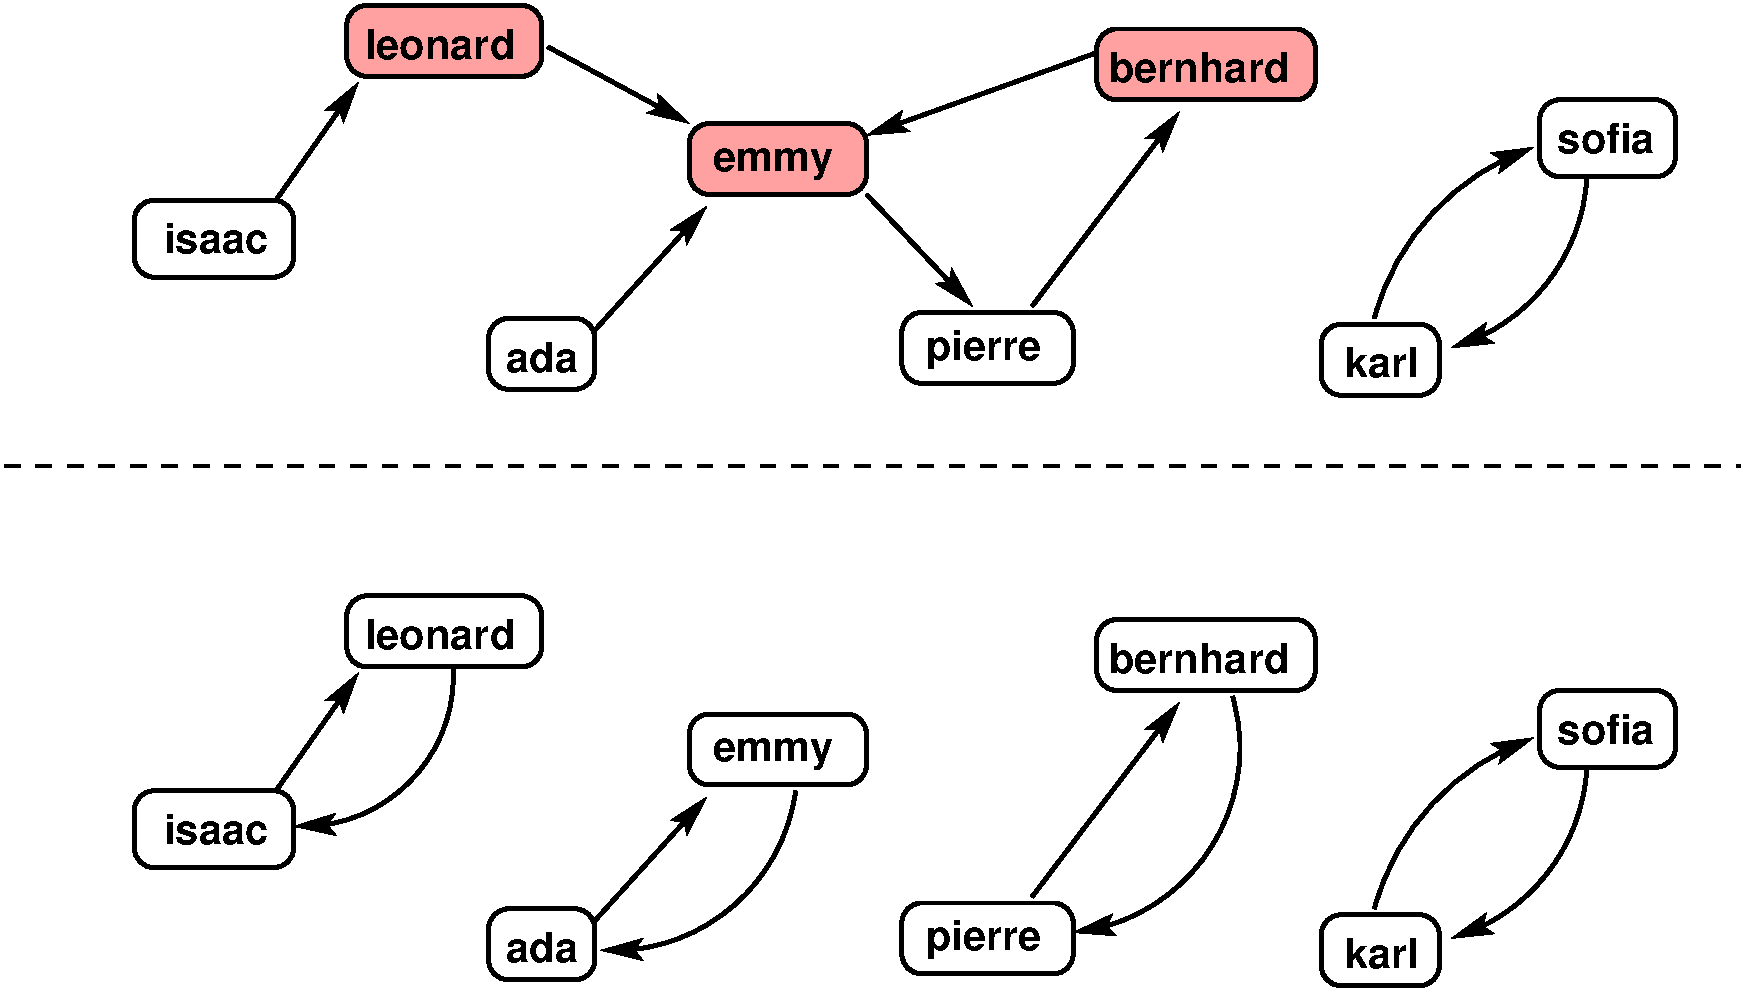
\includegraphics[width=0.5\textwidth]{polygonfig.pdf}
\end{center}

Pirmais paraugs ir ilustrēts augstāk redzamajā attēlā. Attēla augšējā daļa parāda sākotnējo mīlas situāciju,
kur bulta no $s$ uz $t$ nozīmē, ka $s$ sākotnēji mīl $t$, un rozā krāsa izceļ trīs tēlus,
kas jāsašauj ar mīlas bultām, lai iegūtu unikālo optimālo risinājumu. Attēla apakšējā daļa parāda situāciju pēc mīlas bultu izšaušanas.

Otrajā paraugā, kas apmierina trešās grupas ierobežojumus, ir vairāki optimāli risinājumi.
Viens no tiem ir sašaut \texttt{a}, \texttt{b} un \texttt{d} ar mīlas bultām un likt tiem attiecīgi iemīlēties \texttt{b}, \texttt{a} un \texttt{c}.

Trešajā paraugā ir mīlas trīsstūris, kur neatkarīgi no izšauto mīlas bultu skaita, kāds vienmēr nebūs attiecībās.
